\section{Experimental Setup and Evaluation Protocol}
\label{sec:setup}

The comparison contract is the existing experiment plan. Four arms share the
same information pool, action pool and fault domain. Direct numeric comparison
is allowed only on the same denominator and the same charged projection of
\(c=(c_{\mathrm{acq}},c_{\mathrm{comp}},c_{\mathrm{prep}},c_{\mathrm{retry}})\).
Runtime records may retain recovery as a detail, but evaluation folds it into
\(c_{\mathrm{prep}}\) exactly once; it is not a fifth comparison coordinate.
Seven controlled interfaces define scene registration, injection, independent
truth, causal collection, arm execution, validity filtering and evaluation.
Historical captures use only the offline evidence line and are not runnable
scenes or confirmatory truth. The controlled line still depends on an
interactive IUT, confirmed injection, reset evidence, qualified clocks and a
truth generator whose shared components are disclosed.

\begin{itemize}
\item CL-T: predetermined tests; projection \(c_{\mathrm{acq}}\) for tests that
run.
\item CL-A: analysis on pre-allowed records; projection \(c_{\mathrm{comp}}\)
only; no invented sampling cost.
\item CL-TA: frozen collect then analyse; \(c_{\mathrm{acq}}\) and
\(c_{\mathrm{comp}}\) reported separately.
\item CL-LOOP: the CL-TAV session; charge the components that actually run.
\end{itemize}

Truth is typed evaluator-only. It never enters \IFsel, \IFpred, \IFhist{} or
\IFexec; algorithm-visible references are limited to registered initial inputs
and records produced by that arm's own actions. In particular, arms receive the
proposed allowlisted \texttt{algorithmVisibleFields} projection, never the parent
scene record containing the fault plan, truth source, injection confirmation,
validity class or post-hoc adjudication. The projection is a typed member
allowlist containing only scene ID, service scope, registered arm, resource mode
and public-configuration reference; truth, injection, validity, equivalence and
post-hoc members remain forbidden inside the object. Runtime \texttt{IF-EQUIV}
candidate equivalence is distinct from evaluator-side injected-fault
equivalence. The all-attempt ledger retains every registered attempt, including
unconfirmed injection, invalid observation, equivalent or undecided fault,
\texttt{ERROR}, abstention and unconcluded execution. Detection uses a named
valid denominator and a separate answered subset for PASS/FAIL error. Localization
uses confirmed in-domain non-equivalent injections and separately reports
localization-decision coverage, whether the true fault remains or is excluded,
whether an issued singleton is correct, and final \(|H|\). These finite
populations are derived from attempt fields rather than handwritten denominator
tags. Missing truth remains in answered or decision coverage and an explicit
truth-missing flow, but leaves only the relevant truth-scored subset. Thus a valid detection FAIL with
\(H=\{h_1,h_2\}\) is an answered detection outcome but not singleton
localization; \(H=\{h_{\mathrm{normal}}\}\) is not protocol PASS. Mutation
scores exclude only confirmed equivalents while equivalent and undecided counts
and adjudication effort remain visible~\cite{jia2011,gruen2009}.
If no attempt is answered, answered coverage is reported as \(0/N\) for
\(N>0\), whereas answered-conditional error is not applicable. An
\texttt{ERROR}, \texttt{Stop-Empty}, \texttt{Stop-645}, or budget stop cannot
manufacture an answered or singleton-localization decision. Rejected updates
preserve (H) independently of the stop tag; valid empty and singleton updates
force \texttt{Stop-Empty} and \texttt{Stop-Singleton} before later stops.

\begin{figure}[!t]
\centering
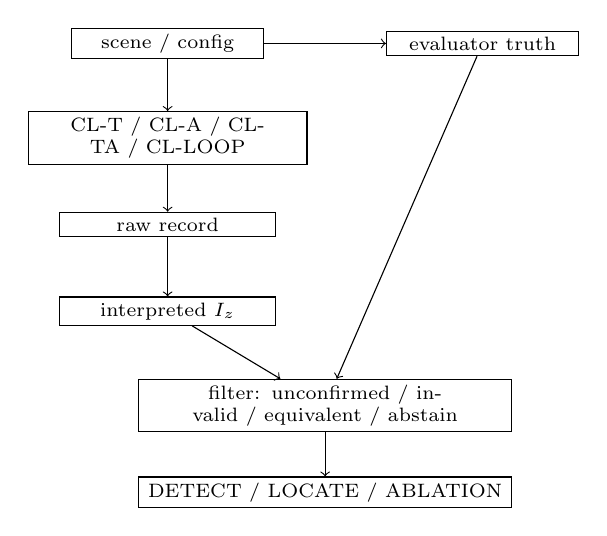
\begin{tikzpicture}[font=\scriptsize,box/.style={draw,align=center,inner sep=2pt}]
\node[box,text width=2.3cm] (scene) at (0,2.6) {scene / config};
\node[box,text width=2.3cm] (truth) at (4.0,2.6) {evaluator truth};
\node[box,text width=3.4cm] (arms) at (0,1.4) {CL-T / CL-A / CL-TA / CL-LOOP};
\node[box,text width=2.6cm] (raw) at (0,0.3) {raw record};
\node[box,text width=2.6cm] (iz) at (0,-0.8) {interpreted \(I_z\)};
\node[box,text width=4.6cm] (filt) at (2.0,-2.0) {filter: unconfirmed / invalid / equivalent / abstain};
\node[box,text width=4.6cm] (met) at (2.0,-3.1) {DETECT / LOCATE / ABLATION};
\draw[->] (scene) -- (arms);
\draw[->] (scene) -- (truth);
\draw[->] (arms) -- (raw);
\draw[->] (raw) -- (iz);
\draw[->] (iz) -- (filt);
\draw[->] (truth) -- (filt);
\draw[->] (filt) -- (met);
\end{tikzpicture}
\caption{Experiment architecture from FIG-CL-TAV-09. Truth meets algorithm
output only at the evaluator filter.}
\label{fig:exp}
\end{figure}

DETECT compares miss and refusal under the same detection budget and the T5
oracle; FIND abort does not waive the 2\,s / 3\,s clocks. LOCATE compares
surviving \(|H|\) and true-fault exclusion on confirmed in-domain injections.
ABLATION uses the registered factors: no feedback (CL-T or CL-TA); Prep/Recover
uncharged; interval versus point-timestamp on the same traces with clocks
fixed; and FIND-abort-as-waiver as a forbidden negative control, not an allowed
algorithm. Sample size remains a named gap.
\phbox{PH-STAT-N}{PUBLICATION-DECISION}{Numeric \(n\), repeats and interval
method freeze at confirmatory registration, not in this draft.}

The implementation-design attachment fixes the accounting contract but not run
parameters. An experimental unit is a unique registered attempt on one base
scene, arm and control/fault construction; packets, events, timestamps and
hypotheses are within-attempt observations. Development, pilot and held-out
lineages are disjoint, and paired arms require independent reset evidence.
Pair eligibility is derived separately for each parent metric and additionally
requires the same registered base scene, seed, construction and contrast,
reciprocal distinct arm identities and distinct confirmed resets;
an unmatched or mismatched row remains in flow accounting but is not imputed.
Eight existing scenario IDs cover normal, WAIT/continue, no-response, abort,
invalid observation, same-key ownership, single-batch comparison and resource
error. Their specification coverage does not establish fault coverage. FIND,
DOWNLOAD, AFDX and runtime integrity capability remain outside first-run
admission. Design review therefore precedes engineering feasibility, pilot,
frozen registration, execution and result acceptance.

For the no-response scenario bound to CRS-M1-00101, the scored trigger is the
data loader receiving a status file that carries an exception delay for the
active operation. A new status strictly before the unresolved expiry endpoint,
or an observed required data-loader abort fallback after expiry, satisfies only
the corresponding continuation or fallback-action proposition. Equality remains
unscored until DEC-CLOCK freezes endpoint inclusivity. This candidate registers
no abort-completion constant: the bound remains null, arbitrary numeric values
are rejected, and finite absence of both events remains unscored. Generic request/response suppression remains a method-only case and is
not scored against CRS-M1-00101; the abort is a prescribed fallback, not a
cancellation waiver.

The registered statistical decision must classify comparisons as primary,
secondary or exploratory and map each primary estimand to its finite domain,
unit, pairing, estimator, interval, applicability and effect scale. Numeric
sample/repeat policy, resource budget and stop priority, and clock/error budget
are separate open decisions with named owners and closure witnesses; none is
selected by this draft. The finite decision table distinguishes a complete
deterministic census, independently randomized attempts, paired units and
clustered units. The independent branch requires independent random assignment,
no dependence and attempt as the unit; the paired and clustered branches require
their respective evidence and units. Missing or inconsistent inputs produce
\texttt{WAIT-DEC-SAMPLE}. Only the independent Bernoulli branch currently names
Clopper--Pearson from a bound direct source; paired and clustered inference remain
method-wait. The examples are hypothetical, not power calculations
or results. One session selects exactly one \texttt{BUDGET} or \texttt{ROUNDS}
mode. A retry cap is an independent execution-safety bound, not a second budget
stop. The timing witness in the design contract uses closed intervals
\(I_{\mathrm{obs}}=[5.0,5.2]~\mathrm{s}\) and
\(I_r=[4.0,5.1]~\mathrm{s}\), whose overlap without containment is
\texttt{INCONCLUSIVE}; containment is PASS and disjointness is FAIL.

Literature methods are not automatically experimental arms. Köhl--Hermanns and
Fränzle~\textit{et al.} are C1 concept comparators because their passive or
non-adaptive testing tasks and observation assumptions differ
\cite{koehl2023,fraenzle2026}. Hu~\textit{et al.} and Miao~\textit{et al.} are
C2 concept comparators, but their controllable-event authority, objective,
observables and stopping rules prevent a fair direct 615A arm without a new
mapping decision~\cite{hu2020,miao2025}. F-LAS, IMA and cockpit-display studies
are scenario or evaluation context, not algorithm baselines
\cite{marques2021,efkemann2011,sartaj2021}. Confirmatory registration must still
freeze the experimental unit, fault construction, equivalence adjudicator,
injection confirmation, clock calibration, stochastic repetition/seeds if any,
and interval/effect-size method; no literature percentage selects those values
\cite{arcuri2011}.
